\documentclass[11pt]{standalone}
\usepackage{tikz}
\usetikzlibrary{positioning}
\usetikzlibrary{intersections}
\usetikzlibrary{shapes.geometric, shapes.arrows, calc, positioning, arrows.meta}
\usetikzlibrary{calc}
\usetikzlibrary{decorations.text}
\usetikzlibrary{external}
\usetikzlibrary{fit}
\newcommand{\metafont}{\sffamily\fontsize{8}{9}\selectfont}
\usepackage{palatino, helvet, inconsolata}

\begin{document}

    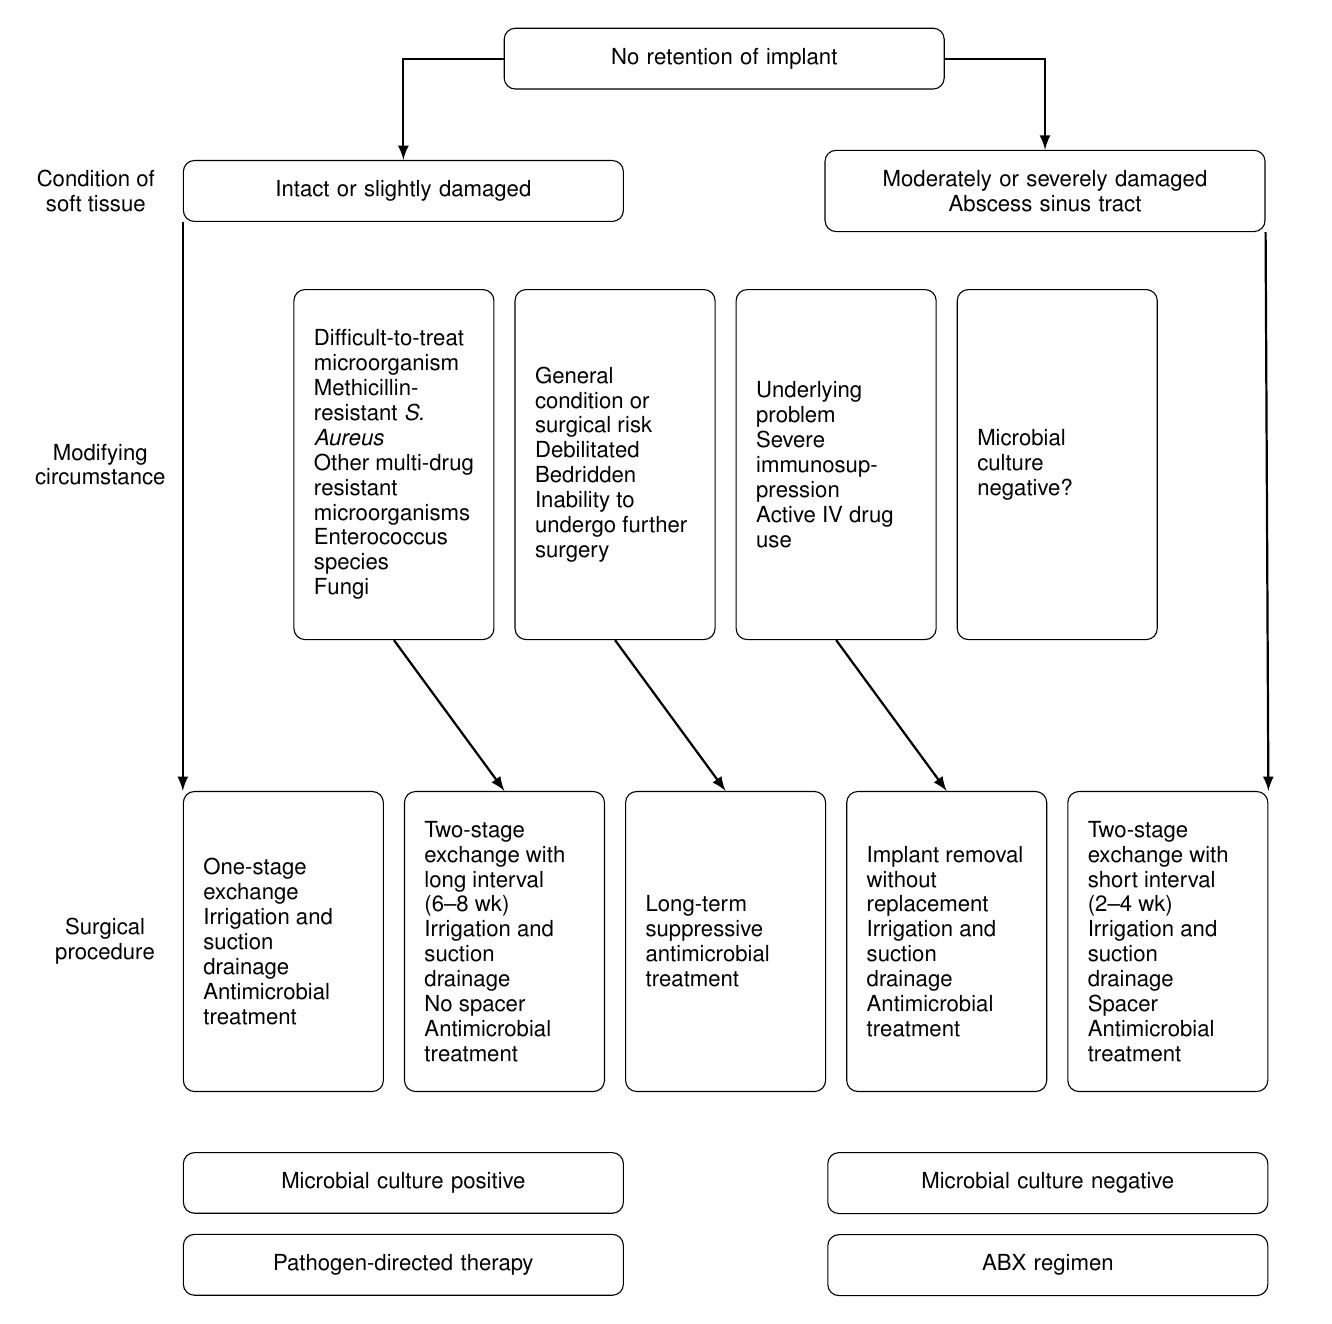
\begin{tikzpicture}[align=center, x=1in, y=-1in, node distance=0.1in]
        \metafont
       \tikzstyle{box} = [
            rectangle,
            draw=black,
            text width=0.8in,
            inner sep=0.1in,
            minimum height=1.5in,
            align=flush left,
            rounded corners
       ]
       \tikzstyle{midbox} = [
           rectangle,
           draw=black,
           text width=0.8in,
           inner sep=0.1in,
           minimum height=1.75in,
           align=flush left,
           rounded corners
       ]
       \tikzstyle{widebox} = [
            rectangle,
            rounded corners,
            draw=black,
            text width=2in,
            inner sep=0.1in
       ]
       \tikzstyle{cross} = [
           inner sep=0pt,
           outer sep=0pt,
       ]
       \tikzstyle{arrow} = [thick, ->, >=latex]
       \node (noretention) at (0,0) [widebox] {No retention of implant};
       \node (x) [cross, below=0.5in of noretention] {};
       \node (intact) [widebox, left=2.7in of x, anchor=west] {Intact or slightly damaged};
       \node (damaged) [widebox, right=2.7in of x, anchor=east] {Moderately or severely damaged\\Abscess sinus tract};
        
       \node (onestage) [box, below=3in of intact.west, anchor=north west] {One-stage exchange\\Irrigation and suction drainage\\Antimicrobial treatment};
       \node (twostage) [box, right=of onestage.north east, anchor=north west] {Two-stage exchange with long interval (6--8 wk)\\Irrigation and suction drainage\\No spacer\\Antimicrobial treatment};
       \node (longterm) [box, right=of twostage.north east, anchor=north west] {Long-term suppressive antimicrobial treatment};
       \node (implant) [box, right=of longterm.north east, anchor=north west] {Implant removal without replacement\\Irrigation and suction drainage\\Antimicrobial treatment};
       \node (twostage2) [box, right=of implant.north east, anchor=north west] {Two-stage exchange with short interval (2--4 wk)\\Irrigation and suction drainage\\Spacer\\Antimicrobial treatment};

       \node (x1) [cross] at ($(onestage.east)!0.5!(twostage.west)$) {};
       \node (x2) [cross] at ($(twostage.east)!0.5!(longterm.west)$) {};
       \node (x3) [cross] at ($(longterm.east)!0.5!(implant.west)$) {};
       \node (x4) [cross] at ($(implant.east)!0.5!(twostage2.west)$) {};

       \node (difficult) [midbox, above=1.5in of x1] {Difficult-to-treat microorganism\\Methicillin-resistant \emph{S.\ Aureus}\\Other multi-drug resistant microorganisms\\Enterococcus species\\Fungi};
       \node (general) [midbox, above=1.5in of x2] {General condition or surgical risk\\Debilitated\\Bedridden\\Inability to undergo further surgery};
       \node (underlying) [midbox, above=1.5in of x3] {Underlying problem\\Severe immunosuppression\\Active IV drug use};
       \node (microbial) [midbox, above=1.5in of x4] {Microbial culture negative?};
       
       \draw[arrow] (noretention) -| (intact);
       \draw[arrow] (noretention) -| (damaged);
       \draw[arrow] (intact.south west) -- (onestage.north west);
       \draw[arrow] (damaged.south east) -- (twostage2.north east);
       \draw[arrow] (difficult.south) -- (twostage.north);
       \draw [arrow] (general.south) -- (longterm.north);
       \draw [arrow] (underlying.south) -- (implant.north);

       \node [left=of intact] {Condition of\\soft tissue};
       \node [left=0.6in of difficult] {Modifying\\circumstance};
       \node [left=of onestage] {Surgical\\procedure};

        \node (positive) [widebox, below=0.3in of onestage.south west, anchor=north west] {Microbial culture positive};
        \node (pathogen) [widebox, below=of positive] {Pathogen-directed therapy};
        \node (negative) [widebox, below=0.3in of twostage2.south east, anchor=north east] {Microbial culture negative};
        \node (abx) [widebox, below=of negative] {ABX regimen};
	   \node (rightwhitespace) [right=0.1in of abx.east] {};
    \end{tikzpicture}
\end{document}